\chapter{Methods}
\label{cha:1}

\section{Dataset and Features}
This project uses the NSL-KDD dataset, a publicly available benchmark dataset for intrusion detection research \cite{tavallaee2009detailed}. NSL-KDD was introduced by Tavallaee et al. as a cleaned and improved version of the original KDD Cup 1999 dataset, addressing major shortcomings such as redundant records and biased attack distributions that previously led to overly optimistic detection results. The dataset is freely accessible via Kaggle and is widely used for evaluating and comparing machine-learning-based intrusion detection systems \cite{abrar2020machine}. The purpose of the NSL-KDD dataset is to support supervised classification of network traffic into normal and malicious behavior. Each data instance represents a single network connection and is described by a fixed set of features capturing various aspects of network activity. The classification task can be formulated either as binary classification (normal vs. attack) or as multi-class classification, where attacks are grouped into four main categories: Denial of Service (DoS), Probe, Remote-to-Local (R2L), and User-to-Root (U2R), in addition to the Normal class \cite{hegde2024intrusion}.

The dataset consists of 125,973 samples in the training set (KDDTrain+) and 22,544 samples in the test set (KDDTest+), for a total of five classes. The class distribution is highly imbalanced, with DoS attacks dominating the dataset, while R2L and especially U2R attacks are extremely rare. This imbalance reflects realistic attack distributions but also introduces challenges for model training and evaluation, particularly in the multi-class setting \cite{hong2021machine}. Each network connection is described by 41 features, composed of a mix of numeric, categorical, and binary attributes \cite{tavallaee2009detailed}. These include basic connection features (e.g., duration, protocol type, service, flag), content-based features (e.g., number of failed login attempts, file creation counts), and traffic-based features computed over time windows (e.g., connection counts, error rates, and bytes sent or received) \cite{tavallaee2009detailed}. The raw data is stored in text (.txt) format, with each row corresponding to a single connection record.

Figure \ref{fig:combined_class} illustrates the class distribution of the NSL-KDD dataset for both the training and test splits. Severe class imbalance is evident in both partitions, with Normal and DoS traffic dominating the data, while R2L and U2R attacks occur extremely rarely \cite{tavallaee2009detailed}.


\begin{figure}[htbp]
    \centering
    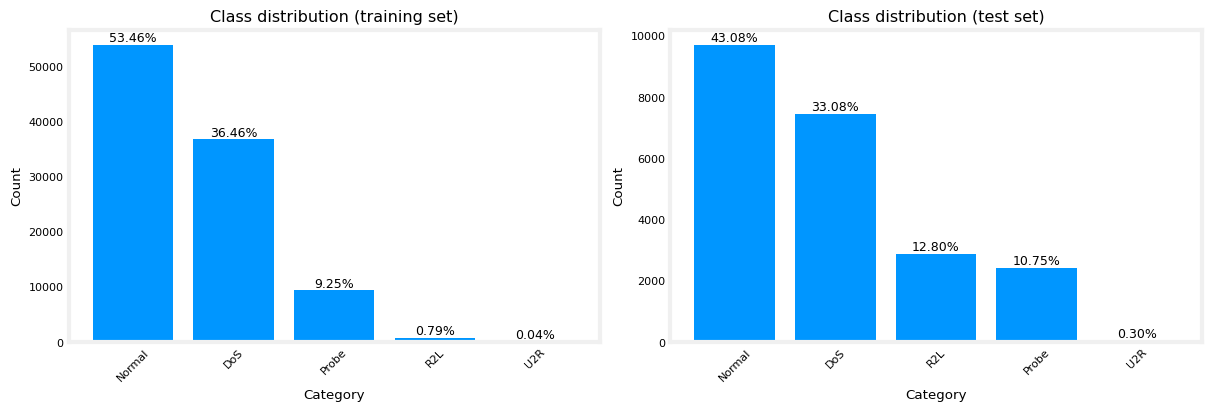
\includegraphics[width=0.9\textwidth]{combined_class.png}
    \caption{Class distribution training vs test}
    \label{fig:combined_class}
\end{figure}

Importantly, the test set exhibits a different class composition than the training set. Although Normal and DoS remain the majority classes, the relative proportions of Probe and R2L attacks increase substantially in the test split. This shift reflects the intentional design of NSL-KDD, in which the test data includes attack types and distributions that are absent or under-represented during training in order to evaluate generalization to previously unseen intrusions \cite{tavallaee2009detailed}. This imbalance and distribution shift have two important implications. First, accuracy alone is a misleading evaluation metric, as strong performance on majority classes can mask poor detection of rare but security-critical attack types such as R2L and U2R. Second, models trained on the imbalanced training data are inherently biased toward dominant classes, making generalization to the test set more challenging. Consequently, the experimental evaluation emphasizes macro-averaged metrics, minority-class recall, and confusion-matrix analysis, and motivates the use of class-weighted learning and more expressive, non-linear models.

Prior to model training, several preprocessing and feature engineering steps are applied. Categorical features, including \texttt{protocol\_type}, \texttt{service}, and \texttt{flag}, are transformed using one-hot encoding, treating categories as nominal variables without imposing an artificial ordinal structure. Continuous features are standardized using z-score normalization (\texttt{StandardScaler}). To prevent data leakage, all preprocessing steps are fitted exclusively on the training subset and subsequently applied unchanged to the validation and test sets. Unseen categorical values in the validation or test data are handled by the encoder’s \texttt{ignore-unknown} implementation. The \texttt{difficulty\_level} attribute introduced by Tavallaee et al. is excluded, as it represents meta-information rather than a network-traffic feature \cite{tavallaee2009detailed}.

Furthermore, different model families may benefit from different feature representations. Tree-based models for example, can operate directly on ordinally encoded categorical variables, while linear and neural models typically require one-hot encodings. However, to ensure a fair and consistent comparison across the three models, a single unified preprocessing pipeline is used for all experiments. This design choice prioritizes consistency and comparability over model-specific optimization. As a result, performance differences can be attributed mainly to the modeling approaches rather than to differences in feature representation. In practice, this unified dense representation primarily affects training efficiency for the Logistic Regression implementation due to the increased feature dimensionality introduced by one-hot encoding. Random Forest and Neural Network training proceed under the same feature representation without requiring separate preprocessing variants.

For model evaluation, the official \texttt{KDDTrain+} dataset is split into training and validation subsets, with the training subset used for parameter estimation and the validation subset used for model selection. The official \texttt{KDDTest+} dataset is reserved exclusively for final evaluation. Notably, the test set contains attack types that are absent from the training data, providing a challenging benchmark for assessing generalization to previously unseen attacks \cite{tavallaee2009detailed}. Strict separation between training, validation, and test sets is applied for all models to obtain an unbiased estimate of model performance. Finally, while the preprocessing pipeline could be made fully reproducible by persisting fitted encoders and scalers using tools such as \texttt{joblib}, this project prioritizes conceptual clarity over production-level delivery. As a result, some best practices, such as persistent transformers, configuration files, and extensive exception handling, are omitted. In a real-world deployment scenario, need for robustness, maintainability, and reproducibility would be essential components of the data-processing workflow.

\section{Models}
\label{sec:models}

The project applies three machine-learning model families to the NSL-KDD intrusion detection task: Logistic Regression, Random Forest, and Neural Networks. These models include linear, ensemble-based, and non-linear approaches, enabling a structured comparison of interpretational capacity, robustness to (severe) class imbalance and generalization behavior, as often recommended in intrusion-detection benchmarking studies \cite{abrar2020machine, hegde2024intrusion, hong2021machine}. All models are trained and evaluated using consistent data splits and evaluation protocols to ensure comparability. Model performance is assessed using accuracy, macro-averaged F1-score, per-class recall, and confusion matrices. For binary classification tasks, ROC curves and AUC scores are additionally computed. Macro-averaged metrics are emphasized due to the strong class imbalance present in NSL-KDD \cite{abrar2020machine, tavallaee2009detailed}. In addition to standard macro recall across all five classes, we also report attack-only macro recall (i.e. excluding Normal class) to better reflect performance across attack categories. This avoids the metric being dominated by the comparatively easy Normal class and provides a clearer view of attack-type sensitivity under class imbalance. No automated hyperparameter search (e.g. grid search or random search) was performed. Instead, model and training hyperparameters were selected through iterative, validation-driven refinement: candidate settings were chosen based on standard defaults and prior literature, then adjusted using validation-set performance and training diagnostics. This approach maintains methodological transparency while keeping the experimental scope aligned with the project constraints.

\subsection{Logistic Regression}
Logistic Regression serves as the baseline model and is directly adapted from the course lab assignments. Its primary objectives are to establish a transparent reference point, validate the preprocessing pipeline, and provide interpretable insights into feature relevance. Logistic Regression has frequently been used as a baseline for NSL-KDD due to its simplicity and interpretability \cite{abrar2020machine, hegde2024intrusion}. For binary classification, it models the probability of intrusion as follows, where $\sigma$ denotes the sigmoid function. Model parameters are optimized by minimizing cross-entropy loss using gradient-based optimization.
\begin{equation}
    P(y=1|x) = \sigma(w^T x + b) = \frac{1}{1 + e^{-(w^T x + b)}}
\end{equation}
The original lab implementation was extended in two important ways. First, class-weighted training was introduced by augmenting the loss and gradient computations with a sample-weight term. This allows training errors on minority classes to be penalized more heavily, partially compensating for the severe imbalance between frequent attacks (e.g., DoS) and rare categories (e.g., R2L and U2R). This approach is widely used to mitigate class imbalance in intrusion detection, where rare attack categories would otherwise have negligible influence on the loss function \cite{abrar2020machine, hong2021machine}. Second, multi-class support was added using a One-vs-Rest (OvR) strategy, a standard extension of binary classifiers for multi-class intrusion detection tasks \cite{hegde2024intrusion}. For a problem with $K$ classes, OvR trains $K$ independent binary classifiers, each distinguishing one class from all others. During inference, all classifiers are evaluated and the class associated with the highest logit value is selected. Stratified k-fold cross-validation was applied only for the binary Logistic Regression baseline to assess robustness under class imbalance. For Random Forest and Neural Network models, evaluation relied on the fixed train/validation split for model selection and the held-out test set for final assessment.

Evaluation of Logistic Regression is performed on a validation set using accuracy and macro-F1 as primary metrics. For the binary formulation, ROC curves and AUC scores are computed using the predicted probabilities from the sigmoid output, as commonly reported in prior NSL-KDD studies \cite{abrar2020machine, hong2021machine}. In addition, stratified k-fold cross-validation is applied in the binary setting to assess robustness across different data partitions while preserving class proportions. In the multi-class setting, raw (non-normalized) confusion matrices are used to analyze absolute error patterns, and top-k accuracy is computed to assess ranking behavior across class logits.

\subsection{Random Forest}
Random Forest (RF) is selected as the primary non-linear model due to its strong empirical performance on NSL-KDD and to its ability to model complex feature interactions, handle mixed feature types, and reduce overfitting through ensemble averaging \cite{abrar2020machine, hegde2024intrusion, hong2021machine}. A Random Forest consists of an ensemble of decision trees trained on bootstrapped samples of the data, where each split considers only a random subset of features. Final predictions are obtained by majority voting across trees. 



The objectives of the Random Forest model are to improve multi-class detection performance relative to linear models, identify informative features, and build a more expressive classifier without excessive overfitting. RF is deliberately used in two distinct stages. In the first stage, an RF model is trained on the full 41-feature dataset to compute feature importance scores, a commonly used technique for feature ranking in intrusion detection \cite{hegde2024intrusion, hong2021machine}. This model is used exclusively for feature ranking and not for final prediction. Based on these rankings, a reduced subset of the most informative features is selected. In the second stage, a new RF model is trained solely on this reduced feature set to serve as the predictive classifier. This two-stage approach enables an explicit evaluation of feature selection effects while maintaining a consistent learning algorithm. Class imbalance is addressed using class-weighted splitting criteria, as recommended in ensemble-based intrusion detection studies \cite{abrar2020machine, hong2021machine}. Evaluation focuses on accuracy, macro-F1 score, and confusion matrices in both multi-class and binary formulations. A binary Random Forest model is additionally trained to isolate the fundamental intrusion-detection capability independent of category-level imbalance.

In our implementation, Random Forest models are trained with 300 trees and a fixed random seed (\texttt{random\_state = 42}) to ensure reproducibility. Trees are allowed to grow without an explicit depth limit (\texttt{max\_depth = None}), while training is parallelized across CPU cores (\texttt{n\_jobs = -1}). Class imbalance is addressed through class-weighted learning: the multi-class feature selection Random Forest uses \texttt{class\_weight = "balanced\_subsample"}, which recomputes weights on each bootstrap sample, whereas the binary Random Forest uses \texttt{class\_weight = "balanced"}, which derives weights from global class frequencies.

\subsection{Neural Networks}
Although neural networks are not always necessary or consistently superior to classical machine-learning techniques on intrusion-detection datasets, their ability to learn higher-order feature interactions makes them a valuable comparison point \cite{ali2025deep, rawat2019intrusion}. Neural networks are therefore introduced as a third modeling family to assess whether their greater representational capacity provides advantages beyond linear and tree-based methods, as is often investigated in the intrusion-detection literature \cite{abrar2020machine, ali2025deep, rawat2019intrusion}. Fully connected feed-forward architectures are used, which are frequently applied to NSL-KDD and related datasets \cite{abrar2020machine, hong2021machine, ali2025deep}.



Several neural-network variants are evaluated to study the effects of regularization and imbalance-aware learning. The baseline multi-class model applies dropout regularization. Model 3MCv2 introduces L1 regularization, while Model 3MCv3 incorporates class weighting at the loss level to address class imbalance. An early stopping mechanism is applied based on validation loss. Binary neural-network variants mirror the multi-class configurations and are trained using binary cross-entropy loss. All Neural Network models use two hidden layers (128 and 64 units) with ReLU activations and dropout regularization (\texttt{Dropout = 0.3}). Multi-class models use a softmax output layer and are trained with sparse categorical cross-entropy using integer-encoded class labels. Training uses the Adam optimizer with mini-batches of 64 samples for up to 50 epochs. For binary neural-network models, decision thresholds are selected based on validation-set precision–recall characteristics, with the threshold maximizing macro-averaged F1-score used for final evaluation.